
\de{ĐỀ THI HỌC KỲ I NĂM HỌC 2022-2023}{Trường THPT CHUYÊN LƯƠNG THẾ VINH - ĐỒNG NAI}
\begin{center}
	\textbf{PHẦN 1 - TRẮC NGHIỆM}
\end{center}
\Opensolutionfile{ans}[ans/ans]
%Câu 1...........................
\begin{ex}%[0H2B2-1]%[Dự án đề kiểm tra HKI NH22-23- Tên GV]%[Chuyên Lương Thế Vinh Đồng Nai]
Cho hình vuông $ABCD$ có cạnh bằng $a$. Khi đó $\left|\overrightarrow{AC}+\overrightarrow{BD}\right|$ bằng
	\choice
	{\True $2a$}
	{$2a\sqrt{2}$}
	{$0$}
	{$a$}
	\loigiai{
\immini 
{
Ta có $\left|\overrightarrow{AC}+\overrightarrow{BD}\right|=2\left|\overrightarrow{AO}+\overrightarrow{OD}\right|=2\left|\overrightarrow{AD}\right|=2a$.
}
{
\begin{tikzpicture}[font=\footnotesize,line join=round, line cap=round,>=stealth,scale=.8]
	\path 
	(0,0)coordinate(A)++(0:3)coordinate(B)++(-90:3)coordinate(C)++(180:3)coordinate(D)
	($(A)!.5!(C)$)coordinate(O)
	;
	\draw 
	(A)--(B)--(C)--(D)--cycle
	;
	\draw [->](A)--(C);
	\draw [->](B)--(D);
	\foreach \x/\g in {A/90,B/90,C/-90,D/-90,O/90}\fill[black](\x) circle(1pt)+(\g:.3)node{$\x$};	
\end{tikzpicture}
}
	}
\end{ex}
%Câu 2...........................
\begin{ex}%[0D2B2-2]%[Dự án đề kiểm tra HKI NH22-23- Tên GV]%[Chuyên Lương Thế Vinh Đồng Nai]
	Trong mặt phẳng $Oxy$, hai đường thẳng $d_1\colon -2x+y-1=0$ và $d_2\colon x+3y-4=0$ chia mặt phẳng thành $4$ miền được đặt tên như hình vẽ. Trong các miền này, miền nào là miền nghiệm của hệ bất phương trình $\heva{&-2x+y-1\ge 0\\&x+3y-4\le 0}$?
	\begin{center}
		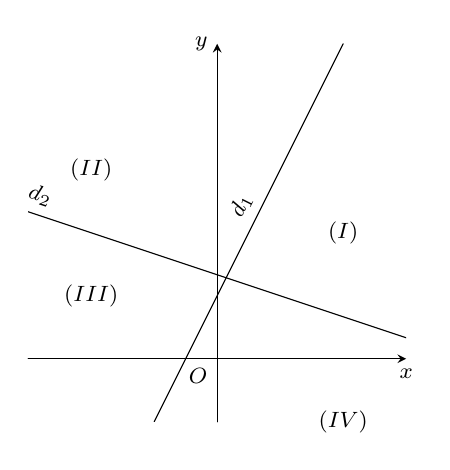
\begin{tikzpicture}[font=\footnotesize,line join=round, line cap=round,>=stealth,scale=.8]
			\begin{scope}
				\clip (-3,-1) rectangle (3,5);
				\draw (2,5)--(-1,-1) node [pos=0.45, above, sloped] {$d_1$};
				\draw (-11,5)--(7,-1) node [pos=0.45, above, sloped] {$d_2$};
			\end{scope}
			\draw[->] (-3,0)--(3,0) node[below]{$x$};
			\draw[->] (0,-1)--(0,5) node[left]{$y$};
			\draw (0,0) node[below left]{$O$}
			(2,2)node{$(I)$}
			(-2,3)node{$(II)$}
			(-2,1)node{$(III)$}
			(2,-1)node{$(IV)$}			
			;
		\end{tikzpicture}
	\end{center}
	\choice
	{Miền $(IV)$}
	{Miền $(I)$}
	{Miền $(II)$}
	{\True Miền $(III)$}
	\loigiai{
	\immini
	{
	Miền nghiệm của bất phương trình $-2x+y-1\ge 0$ là nửa mặt phẳng kể cả bờ là đường thẳng $d_1$ và không chứa $O$.\\
	Miền nghiệm của bất phương trình $-x+3y-4\le 0$ là nửa mặt phẳng kể cả bờ là đường thẳng $d_2$ và chứa $O$.\\
	Do đó, miền nghiệm của hệ bất phương trình đã cho là miền $(III)$.
}
{
	\begin{tikzpicture}[font=\footnotesize,line join=round, line cap=round,>=stealth,scale=.8]
	\begin{scope}
		\clip (-3,-1) rectangle (3,5);
		\fill[pattern=grid] (-4,-7)--(4,-7)--(4,9)--cycle;
		\fill[pattern=grid] (-12,5.33)--(8,5.33)--(8,-1.33)--cycle;
		\draw (2,5)--(-1,-1) node [pos=0.45, above, sloped] {$d_1$};
		\draw (-11,5)--(7,-1) node [pos=0.45, above, sloped] {$d_2$};
	\end{scope}
	\draw[->] (-3,0)--(3,0) node[below]{$x$};
	\draw[->] (0,-1)--(0,5) node[left]{$y$};
	\draw (0,0) node[below left]{$O$};
\end{tikzpicture}
}
	}
\end{ex}
%Câu 3...........................
\begin{ex}%[0D3B2-1]%[Dự án đề kiểm tra HKI NH22-23- Tên GV]%[Chuyên Lương Thế Vinh Đồng Nai]
	Xác định các giá trị $a$, $b$ để hàm số $y=x^2+ax+b$ có đồ thị $(P)$ như hình vẽ
	\begin{center}
		\begin{tikzpicture}[font=\footnotesize,line join=round, line cap=round,>=stealth,scale=.8]
			\draw[->] (-3.1,0)--(3.1,0) node[below left] {$x$};
			\draw[->] (0,-2.6)--(0,3.1) node[below left] {$y$};
			\draw (0,0) node [below left] {$O$};
			\foreach \x in {1}
			\draw[thin] (\x,1pt)--(\x,-1pt) node [below] {$\x$};
			\foreach \y in {-2}
			\draw[thin] (1pt,\y)--(-1pt,\y) node [left] {$\y$};
			\begin{scope}
				\clip (-3,-2.5) rectangle (3,3);
				\draw[samples=200,domain=-3:2,smooth,variable=\x] plot (\x,{1*(\x)^2+1*(\x)+-2});
			\end{scope}
		\end{tikzpicture}
	\end{center}
	\choice
	{$a=2$; $b=1$}
	{$a=2$; $b=-2$}
	{\True $a=1$; $b=-2$}
	{$a=1$; $b=2$}
	\loigiai{
	Đồ thị hàm số đi qua điểm $A(1;0)$ và $(0;-2)$ nên ta có hệ phương trình
	$$\heva{&1+a+b=0\\&b=-2}\Leftrightarrow\heva{&a=1\\&b=-2.}$$
	}
\end{ex}
%Câu 4...........................
\begin{ex}%[0H3B1-4]%[Dự án đề kiểm tra HKI NH22-23- Tên GV]%[Chuyên Lương Thế Vinh Đồng Nai]
	Trong mặt phẳng $Oxy$, cho hai véc-tơ $\overrightarrow{a}$, $\overrightarrow{b}$ không cùng phương. Biết rằng hai véc-tơ $\overrightarrow{u}=3\overrightarrow{a}-2\overrightarrow{b}$ và $\overrightarrow{v}=(x+1)\overrightarrow{a}+4\overrightarrow{b}$ cùng phương với nhau. Khi đó giá trị của $x$ bằng
	\choice
	{$5$}
	{\True $-7$}
	{$-6$}
	{$7$}
	\loigiai{
		Hai véc-tơ cùng phương nên $\dfrac{x+1}{3}=\dfrac{4}{-2}\Leftrightarrow x+1=-6\Leftrightarrow x=-7$.
	}
\end{ex}
%Câu 5...........................
\begin{ex}%[0D3Y2-1]%[Dự án đề kiểm tra HKI NH22-23- Tên GV]%[Chuyên Lương Thế Vinh Đồng Nai]
	Hàm số nào sau đây là hàm số bậc hai theo biến $x$?
	\choice
	{$y=\dfrac{x+2}{x-1}$}
	{$y=x^3-2x^2+x$}
	{\True $y=x^2-x+1$}
	{$y=\sqrt{x^2-3}$}
	\loigiai{
	Hàm số bậc hai có dạng $y=ax^2+bx+c$ với $a\ne 0$.\\
	Do đó, $y=x^2-x+1$ là một hàm số bậc hai.
	}
\end{ex}
%Câu 6...........................
\begin{ex}%[0D1Y3-1]%[Dự án đề kiểm tra HKI NH22-23- Tên GV]%[Chuyên Lương Thế Vinh Đồng Nai]
	Tập hợp $(2;10]\cap [8;15]$ bằng tập hợp nào sau đây?
	\choice
	{$(10;15]$}
	{$(2;8)$}
	{$(2;15]$}
	{\True $[8;10]$}
	\loigiai{
	Ta có $(2;10]\cap [8;15]=[8;10]$.
	}
\end{ex}
%Câu 7...........................
\begin{ex}%[0D1B1-3]%[Dự án đề kiểm tra HKI NH22-23- Tên GV]%[Chuyên Lương Thế Vinh Đồng Nai]
	Mệnh đề phủ định của mệnh đề $P\colon$\lq\lq$\forall x\in\mathbb{R}:x^2+x+2>0$\rq\rq\, là
	\choice
	{$\overline{P}\colon$\lq\lq$\forall x\notin\mathbb{R}:x^2+x+2>0$\rq\rq}
	{\True $\overline{P}\colon$\lq\lq$\exists x\notin\mathbb{R}:x^2+x+2\le 0$\rq\rq}
	{$\overline{P}\colon$\lq\lq$\exists x\in\mathbb{R}:x^2+x+2\le 0$\rq\rq}
	{$\overline{P}\colon$\lq\lq$\forall x\in\mathbb{R}:x^2+x+2\le 0$\rq\rq}
	\loigiai{
		Mệnh đề phủ định của mệnh đề $P\colon$\lq\lq$\forall x\in\mathbb{R}:x^2+x+2>0$\rq\rq\, là $\overline{P}\colon$\lq\lq$\exists x\notin\mathbb{R}:x^2+x+2\le 0$\rq\rq.
	}
\end{ex}
%Câu 8...........................
\begin{ex}%[0H1B2-2]%[Dự án đề kiểm tra HKI NH22-23- Tên GV]%[Chuyên Lương Thế Vinh Đồng Nai]
	Cho tam giác $ABC$ có bán kính đường tròn nội tiếp bằng $2$ và diện tích bằng $30$. Chu vi tam giác $ABC$ bằng
	\choice
	{$12$}
	{$6$}
	{$15$}
	{\True $30$}
	\loigiai{
	Ta có $S=pr\Rightarrow p=\dfrac{S}{r}=\dfrac{30}{2}=15$.\\
	Do đó, chu vi tam giác $ABC$ là $2p=30$.
	}
\end{ex}
%Câu 9...........................
\begin{ex}%[0D3Y2-3]%[Dự án đề kiểm tra HKI NH22-23- Tên GV]%[Chuyên Lương Thế Vinh Đồng Nai]
	Trong mặt phẳng $Oxy$, điểm nào sau đây thuộc đồ thị hàm số $y=2x^2-x+3$?
	\choice
	{\True $(3;18)$}
	{$(1;5)$}
	{$(0;-3)$}
	{$(-2;11)$}
	\loigiai{
	Ta có $2\cdot (3)^2-3+3=18$ nên $(3;18)$ thuộc đồ thị hàm số $y=2x^2-x+3$.
	}
\end{ex}
%Câu 10...........................
\begin{ex}%[0D3Y2-2]%[Dự án đề kiểm tra HKI NH22-23- Tên GV]%[Chuyên Lương Thế Vinh Đồng Nai]
	Hàm số $y=-x^2+4x-5$ đồng biến trên khoảng nào sau đây?
	\choice
	{$(-\infty;4)$}
	{\True $(-\infty;2)$}
	{$(-2;+\infty)$}
	{$(2;+\infty)$}
	\loigiai{
	Ta có $x=-\dfrac{b}{a}=2$ là trục đối xứng của đồ thị hàm số đã cho.\\
	Bảng biến thiên
	\begin{center}
		
\begin{tikzpicture}
			\tkzTabInit[lgt=1.2,espcl=3]
			{$x$/1,$y$/2}
			{$-\infty$,$2$,$+\infty$}
			\tkzTabVar{-/$-\infty$,+/$-1$,-/$-\infty$}
		\end{tikzpicture}
	\end{center}
	Hàm số đồng biến trên khoảng $(-\infty;2)$.
	}
\end{ex}
%Câu 11...........................
\begin{ex}%[0D2B2-3]%[Dự án đề kiểm tra HKI NH22-23- Tên GV]%[Chuyên Lương Thế Vinh Đồng Nai]
	Một cửa hàng với số vốn $570$ triệu đồng dự định nhập về hai loại tivi $A$ và $B$ để bán, với giá nhập về của mỗi chiếc lần lượt là $4$ triệu đồng và $6$ triệu đồng. Theo ước tính, nhu cầu tivi hàng tháng không vượt quá $100$ chiếc. Nếu gọi $x$, $y$ (chiếc) lần lượt gọi là số lượng ti vi loại $A$ và $B$ mà cửa hàng nhập về, hệ phương trình nào sau đây thể hiện các điều kiện ràng buộc của $x$ và $y$?
	\choice
	{$\heva{&x>0\\&y>0\\&x+y\le 100\\&4x+6y\le 570}$}
	{\True $\heva{&x\ge 0\\&y\ge 0\\&x+y\le 100\\&4x+6y\le 570}$}
	{$\heva{&x\ge 0\\&y\ge 0\\&x+y\ge 100\\&4x+6y\ge 570}$}
	{$\heva{&x>0\\&y>0\\&x+y< 100\\&4x+6y< 570}$}
	\loigiai{
	Do cửa hàng có thể không nhập hàng nên $x\ge 0$ và $y\ge 0$.\\
	Do nhu cầu không vượt quá $100$ chiếc nên $x+y\le 100$.\\
	Cửa hàng có số vốn $570$ triệu nên số tiền mua hàng $4x+6y\le 570$.\\
	Vậy hệ phương trình thỏa mãn các điều kiện ràng buộc là $\heva{&x\ge 0\\&y\ge 0\\&x+y\le 100\\&4x+6y\le 570.}$
	}
\end{ex}
%Câu 12...........................
\begin{ex}%[0H2Y1-2]%[Dự án đề kiểm tra HKI NH22-23- Tên GV]%[Chuyên Lương Thế Vinh Đồng Nai]
	Phát biểu nào sau đây là \textbf{sai}?
	\choice
	{Hai véc-tơ đối nhau thì cùng phương}
	{Hai véc-tơ ngược hướng thì cùng phương}
	{Hai véc-tơ bằng nhau thì cùng hướng}
	{\True Hai véc-tơ cùng phương thì cùng hướng}
	\loigiai{
	Hai véc-tơ cùng phương thì cùng hướng là phát biểu sai.
	}
\end{ex}
%Câu 13...........................
\begin{ex}%[0H2Y4-2]%[Dự án đề kiểm tra HKI NH22-23- Tên GV]%[Chuyên Lương Thế Vinh Đồng Nai]
	Cho hai véc-tơ $\overrightarrow{a}$, $\overrightarrow{b}$ đều khác véc-tơ-không sao cho $\overrightarrow{a}\cdot\overrightarrow{b}=-\left|\overrightarrow{a}\right|\left|\overrightarrow{b}\right|$. Khi đó góc giữa hai véc-tơ bằng
	\choice
	{$\left(\overrightarrow{a},\overrightarrow{b}\right)=0^\circ$}
	{\True $\left(\overrightarrow{a},\overrightarrow{b}\right)=180^\circ$}
	{$\left(\overrightarrow{a},\overrightarrow{b}\right)=45^\circ$}
	{$\left(\overrightarrow{a},\overrightarrow{b}\right)=90^\circ$}
	\loigiai{
	Ta có $\cos\left(\overrightarrow{a},\overrightarrow{b}\right)=\dfrac{\overrightarrow{a}\cdot\overrightarrow{b}}{\left|\overrightarrow{a}\right|\left|\overrightarrow{b}\right|}=-1$. Suy ra $\left(\overrightarrow{a},\overrightarrow{b}\right)=180^\circ$.
	}
\end{ex}
%Câu 14...........................
\begin{ex}%[0H2B2-4]%[Dự án đề kiểm tra HKI NH22-23- Tên GV]%[Chuyên Lương Thế Vinh Đồng Nai]
	Cho tam giác $ABC$ và điểm $M$ thỏa mãn $\overrightarrow{MB}+\overrightarrow{MC}=\overrightarrow{CM}-\overrightarrow{CA}$. Mệnh đề nào sau đây đúng?
	\choice
	{$M$ là trung điểm đoạn $AB$}
	{$M$ là trung điểm đoạn $AC$}
	{$M$ là trung điểm đoạn $BC$}
	{\True $M$ là trọng tâm tam giác $ABC$}
	\loigiai{
	Ta có
	\allowdisplaybreaks
	\begin{eqnarray*}
		\overrightarrow{MB}+\overrightarrow{MC}=\overrightarrow{CM}-\overrightarrow{CA}&\Leftrightarrow&\overrightarrow{MB}+\overrightarrow{MC}=\overrightarrow{AM}\\
		&\Leftrightarrow&\overrightarrow{MB}+\overrightarrow{MC}+\overrightarrow{MA}=\overrightarrow{0}.
	\end{eqnarray*}
	Do đó, $M$ là trọng tâm tam giác $ABC$.
	}
\end{ex}
%Câu 15...........................
\begin{ex}%[0D3Y1-2]%[Dự án đề kiểm tra HKI NH22-23- Tên GV]%[Chuyên Lương Thế Vinh Đồng Nai]
	Xét hàm số $y=f(x)$ cho bởi bảng sau
	\begin{center}
\begin{tabular}{|c|c|c|c|c|c|}
	\hline
$x$	& $1$ & $2$ & $3$ & $4$ & $5$ \\
	\hline
$f(x)$	& $9$ & $6$ & $7$ & $8$ & $10$ \\
	\hline
\end{tabular}
	\end{center}
Tập xác định của hàm số này là
	\choice
	{$\mathscr{D}=\{6;7;8;9;10\}$}
	{$\mathscr{D}=[1;5]$}
	{\True $\mathscr{D}=\{1;2;3;4;5\}$}
	{$\mathscr{D}=\mathbb{R}$}
	\loigiai{
		Tập xác định của hàm số này là $\mathscr{D}=\{1;2;3;4;5\}$.
	}
\end{ex}
%Câu 16...........................
\begin{ex}%[0D3Y1-3]%[Dự án đề kiểm tra HKI NH22-23- Tên GV]%[Chuyên Lương Thế Vinh Đồng Nai]
	Cho hàm số $y=f(x)=\heva{&x-2\text{ với } x>2\\&1-3x^2\text{ với }x\le 2}$. Giá trị $f(0)$ bằng
	\choice
	{$0$}
	{\True $1$}
	{$2$}
	{$-2$}
	\loigiai{
	Ta có $f(0)=1-3\cdot 0^2=1$.
	}
\end{ex}
%Câu 17...........................
\begin{ex}%[0H1Y2-1]%[Dự án đề kiểm tra HKI NH22-23- Tên GV]%[Chuyên Lương Thế Vinh Đồng Nai]
	Cho tam giác $ABC$ có $BC=a$, $AC=b$, $AB=c$. Mệnh đề nào sau đây là đúng?
	\choice
	{$\cos A=\dfrac{b^2+c^2+a^2}{bc}$}
	{\True $\cos A=\dfrac{b^2+c^2-a^2}{2bc}$}
	{$\cos A=\dfrac{b^2+c^2-a^2}{bc}$}
	{$\cos A=\dfrac{b^2+c^2+a^2}{2bc}$}
	\loigiai{
	Ta có $\cos A=\dfrac{b^2+c^2-a^2}{2bc}$.
	}
\end{ex}
%Câu 18...........................
\begin{ex}%[0H2Y3-1]%[Dự án đề kiểm tra HKI NH22-23- Tên GV]%[Chuyên Lương Thế Vinh Đồng Nai]
	Cho ba điểm $A$, $B$, $C$ thẳng hàng theo thứ tự sao cho $AB=2$, $AC=6$. Đẳng thức nào sau đây đúng?
	\choice
	{$\overrightarrow{BC}=-2\overrightarrow{AB}$}
	{\True $\overrightarrow{BC}=-2\overrightarrow{BA}$}
	{$\overrightarrow{BC}=3\overrightarrow{AB}$}
	{$\overrightarrow{BC}=4\overrightarrow{AB}$}
	\loigiai{
	\immini
	{
	Ta có $\overrightarrow{BC}=-2\overrightarrow{BA}$.
}
{
	\begin{tikzpicture}[font=\footnotesize,line join=round, line cap=round,>=stealth,scale=.8]
\path 
(0,0)coordinate(A)++(0:2)coordinate(B)++(0:4)coordinate(C)
;
\draw 
(A)--(C)
;
\foreach \x/\g in {A/90,B/90,C/90}\fill[black](\x) circle(1pt)+(\g:.3)node{$\x$};	
\end{tikzpicture}
}
	}
\end{ex}
%Câu 19...........................
\begin{ex}%[0D2Y2-2]%[Dự án đề kiểm tra HKI NH22-23- Tên GV]%[Chuyên Lương Thế Vinh Đồng Nai]
	Cặp số nào sau đây là một nghiệm của hệ phương trình $\heva{&2x+y-5<0\\&x-y+7>0}$?
	\choice
	{$(0;10)$}
	{$(10;0)$}
	{\True $(0;-10)$}
	{$(-10;0)$}
	\loigiai{
		Ta có $\heva{&2\cdot 0-10-5<0\\&0-(-10)+7>0}$ nên $(0;-10)$ là nghiệm của hệ phương trình đã cho.
	}
\end{ex}
%Câu 20...........................
\begin{ex}%[0H2Y1-3]%[Dự án đề kiểm tra HKI NH22-23- Tên GV]%[Chuyên Lương Thế Vinh Đồng Nai]
	Cho hình bình hành $ABCD$ tâm $O$. Véc-tơ nào sau đây bằng véc-tơ $\overrightarrow{CO}$?
	\choice
	{$\overrightarrow{AO}$}
	{\True $\overrightarrow{OA}$}
	{$\overrightarrow{BO}$}
	{$\overrightarrow{OC}$}
	\loigiai{
	\immini
{
	Ta có $\overrightarrow{CO}=\overrightarrow{OA}$.
}
{
	\begin{tikzpicture}[font=\footnotesize,line join=round, line cap=round,>=stealth,scale=.8]
		\path 
		(0,0)coordinate(A)++(0:4)coordinate(B)++(230:2)coordinate(C)++(180:4)coordinate(D)
		($(A)!.5!(C)$)coordinate(O)
		;
		\draw 
		(A)--(B)--(C)--(D)--cycle
		;
		\draw [->](C)--(O);
		\draw [->](O)--(A);
		\foreach \x/\g in {A/90,B/90,C/-90,D/-90,O/90}\fill[black](\x) circle(1pt)+(\g:.3)node{$\x$};	
	\end{tikzpicture}
}
	}
\end{ex}
%Câu 21...........................
\begin{ex}%[0D2Y1-2]%[Dự án đề kiểm tra HKI NH22-23- Tên GV]%[Chuyên Lương Thế Vinh Đồng Nai]
	Trong mặt phẳng $Oxy$, cho đường thẳng $\Delta\colon 2x-y+3=0$. Miền nghiệm của bất phương trình $2x-y+3>0$ là
	\choice
	{\True Nửa mặt phẳng không kể bờ $\Delta$, chứa gốc tọa độ $O$}
	{Nửa mặt phẳng kể cả bờ $\Delta$, không chứa gốc tọa độ $O$}
	{Nửa mặt phẳng không kể bờ $\Delta$, không chứa gốc tọa độ $O$}
	{Nửa mặt phẳng kể cả bờ $\Delta$, chứa gốc tọa độ $O$}
	\loigiai{
	Do $2\cdot 0-0+3>0$ nên miền nghiệm của bất phương trình $2x-y+3>0$ là nửa mặt phẳng không kể bờ $\Delta$, chứa gốc tọa độ $O$.
	}
\end{ex}
%Câu 22...........................
\begin{ex}%[0D1Y1-4]%[Dự án đề kiểm tra HKI NH22-23- Tên GV]%[Chuyên Lương Thế Vinh Đồng Nai]
	Tỉ lệ vàng $\varphi$ là một tỉ lệ xuất hiện trong nhiều lĩnh vực như kiến trúc, hội họa, toán học, sinh học,$\ldots$. Biết rằng $\varphi=\dfrac{1+\sqrt{5}}{2}=1{,}618033\ldots$. Xác định số gần đúng của $\varphi$ với độ chính xác $d=0{,}001$.
	\choice
	{$1{,}62$}
	{$1{,}6$}
	{\True $1{,}618$}
	{$1{,}61$}
	\loigiai{
	Số gần đúng của $\varphi$ với độ chính xác $d=0{,}001$ là $1{,}618$.
	}
\end{ex}
%Câu 23...........................
\begin{ex}%[0D1Y1-2]%[Dự án đề kiểm tra HKI NH22-23- Tên GV]%[Chuyên Lương Thế Vinh Đồng Nai]
Một phép đo khối lượng sản phẩm cho kết quả là $100\pm 2$ mg. Gọi $\overline{m}$ (mg) là khối lượng thực của sản phẩm này. Khẳng định nào sau đây là đúng?
	\choice
	{$\overline{m}\in\{98;102\}$}
	{$\overline{m}=2$}
	{$\overline{m}=100$}
	{\True $\overline{m}\in\left[98;102\right]$}
	\loigiai{
	Ta có $\overline{m}\in\left[98;102\right]$.
	}
\end{ex}
%Câu 24...........................
\begin{ex}%[0H2B2-3]%[Dự án đề kiểm tra HKI NH22-23- Tên GV]%[Chuyên Lương Thế Vinh Đồng Nai]
	Cho ba điểm $A$, $B$, $C$ phân biệt. Đẳng thức nào sau đây là \textbf{sai}?
	\choice
	{$\overrightarrow{AB}-\overrightarrow{AC}=\overrightarrow{CB}$}
	{$\overrightarrow{BA}-\overrightarrow{CA}=\overrightarrow{BC}$}
	{$\overrightarrow{AB}+\overrightarrow{BC}=\overrightarrow{AC}$}
	{\True $\overrightarrow{AB}+\overrightarrow{CA}=\overrightarrow{BC}$}
	\loigiai{
	Ta có $\overrightarrow{AB}+\overrightarrow{CA}=\overrightarrow{BC}$ là sai do $\overrightarrow{AB}+\overrightarrow{CA}=\overrightarrow{CB}$.
	}
\end{ex}
%Câu 25...........................
\begin{ex}%[0D2Y2-1]%[Dự án đề kiểm tra HKI NH22-23- Tên GV]%[Chuyên Lương Thế Vinh Đồng Nai]
	Bất phương trình nào sau đây \textbf{không} là bất phương trình bậc nhất hai ẩn?
	\choice
	{$3x-y-2\ge 0$}
	{$2x-7>0$}
	{\True $x-2y^2+3<0$}
	{$x+3y-5\le 0$}
	\loigiai{
		$x-2y^2+3<0$ có bậc hai nên đây không là bất phương trình bậc nhất hai ẩn.
	}
\end{ex}
\Closesolutionfile{ans}
\begin{center}
	\textbf{ĐÁP ÁN}
	\inputansbox{10}{ans/ans}	
\end{center}
\begin{center}
	\textbf{PHẦN 2 - TỰ LUẬN}
\end{center}

\begin{bt}%[0T3B1-2]%[Dự án đề kiểm tra HKI NH22-23- NguyenHuynh]%[Trường THPT Chuyên LTV]
	Tìm tập xác định của các hàm số sau: \begin{enumerate}[a)]
		\item  $y=\sqrt{x-5}+\sqrt{10-x}$.
		\item $y=\dfrac{x+1}{x^2-3 x+2}$.
	\end{enumerate}
	\loigiai{\begin{enumerate}[a)]
			\item  Hàm số xác định khi $\heva{&x-5\ge 0 \\ &10-x \ge 0}$ $\Leftrightarrow \heva{&x\ge 5 \\ &x \le 10.}$ Vậy tập xác định $\mathscr D=\left[5;10\right]$. 
			\item Hàm số xác định khi $x^2-3 x+2\ne 0 \Leftrightarrow \heva{&x\ne 1 \\ &x \ne 2} $. Vậy tập xác định $\mathscr D= \mathbb{R} \backslash \{1;2\}$.
	\end{enumerate}}
\end{bt}

\begin{bt}%[0T3K2-1] %[Dự án đề kiểm tra HKI NH22-23- NguyenHuynh]%[Trường THPT Chuyên LTV]
	Biết rằng hàm số bậc hai $y=m x^2+2 x+n$ có tập giá trị là $(-\infty ; 4]$ và có đồ thị nhận đường thẳng $x=1$ làm trục đối xứng. Xác định các giá trị $m$ và $n$.
	\loigiai{Hàm số bậc hai $y=m x^2+2 x+n$ có tập giá trị là $(-\infty ; 4]$ và có đồ thị nhận đường thẳng $x=1$ làm trục đối xứng nên có đỉnh là $S(1;4)$. Khi đó $$\heva{&x_S=-\dfrac{b}{2a}=-\dfrac{2}{2m}=1 \\ &y_S=m\cdot1^2+2\cdot1+n=4} \Leftrightarrow \heva{&m=-1 \\ &n=3.}$$
	Vậy $m=-1$ và $n=3$.}
\end{bt}
\begin{bt}%[0T5B3-4]%[0T5K4-1]%[Dự án đề kiểm tra HKI NH22-23- NguyenHuynh]%[Trường THPT Chuyên LTV]
	Cho tam giác $A B C$ là tam giác đều có cạnh bằng $a$. 
	\begin{enumerate} [a)]
		\item  Xác định vị trí điểm $N$ sao cho $2 \overrightarrow{A N}=\overrightarrow{N C}$.
		\item  Tính $\overrightarrow{B N}$ theo $\overrightarrow{B A}, \overrightarrow{B C}$.
		\item  Tính tích vô hướng $\overrightarrow{A B} \cdot \overrightarrow{B N}$.
	\end{enumerate}
	\loigiai{\begin{center}
			\begin{tikzpicture}[line cap=round,line join=round,font=\footnotesize,>=stealth,scale=1.1]
				\path	(90:3) coordinate (A) node[shift={(90:1ex)}]{$A$} circle(3pt)
				(210:3) coordinate [label=left:$B$] (B) circle(1pt)
				(-30:3) coordinate [label=right:$C$] (C) circle(1pt)
				($(A)!1/3!(C)$) coordinate [label=right:$N$] (N) circle(1pt);
				\draw (A)--(B)--(C)--(A) (B)--(N);
				\draw[->] (A)--(N); \draw[->] (N)--(C); \draw[->](B)--(N);\end{tikzpicture}
		\end{center}
		\begin{enumerate} [a)]
			\item  Ta có $2 \overrightarrow{A N}=\overrightarrow{N C} \Leftrightarrow 2 \overrightarrow{A N}=\overrightarrow{AC}-\overrightarrow{AN}\Leftrightarrow 3 \overrightarrow{A N}=\overrightarrow{AC}\Leftrightarrow  \overrightarrow{A N}=\dfrac{1}{3}\overrightarrow{AC}$.
			\\Vậy $N$ là điểm thuộc đoạn thẳng $AC$ sao cho $AC=3AN$.
			\item Ta có: $\overrightarrow{B N}=\overrightarrow{BA}+\overrightarrow{A N}=\overrightarrow{BA}+\dfrac{1}{3}\overrightarrow{AC}=\overrightarrow{BA}+\dfrac{1}{3} \left(\overrightarrow{BC}-\overrightarrow{BA}\right)=\dfrac{2}{3}\overrightarrow{BA}+\dfrac{1}{3}\overrightarrow{BC}$.
			\item Ta có $$\begin{aligned}
				\overrightarrow{A B} \cdot \overrightarrow{B N}&=-\overrightarrow{BA}\cdot \left(\dfrac{2}{3}\overrightarrow{BA}+\dfrac{1}{3}\overrightarrow{BC}\right)\\&=-\dfrac{2}{3}BA^2-\dfrac{1}{3}\overrightarrow{ BA} \cdot \overrightarrow{B C}\\&=-\dfrac{2}{3}BA^2-\dfrac{1}{3}BA \cdot BC \cdot \cos60^\circ\\&=-\dfrac{2}{3}a^2-\dfrac{1}{3}a\cdot a \cdot \cos60^\circ\\&=-\dfrac{5}{6}a^2.
			\end{aligned}$$
			Vậy $	\overrightarrow{A B} \cdot \overrightarrow{B N}= -\dfrac{5}{6}a^2$.
	\end{enumerate}}
\end{bt}
\begin{bt}%[0T2B2-3]%[Dự án đề kiểm tra HKI NH22-23- NguyenHuynh]%[Trường THPT Chuyên LTV]
	Ông An dự định làm bánh chưng và bánh tét để bán vào dịp Tết Quý Mão 2023 với giá lần lượt là 130 nghìn và 160 nghìn đồng mỗi chiếc. Biết rằng để làm một chiếc bánh chưng cần $500\mathrm{~g}$ gạo nếp và $150\mathrm{~g}$ thịt, để làm một chiếc bánh tét cần $400\mathrm{~g}$ gạo nếp và $200\mathrm{~g}$ thịt. Tính số lượng bánh mỗi loại để số tiền bán bánh thu được là lớn nhất, biết rằng ông An chỉ sử dụng tối đa $10\mathrm{~kg}$ nếp và $4,2\mathrm{~kg}$ thịt.
	\loigiai{Gọi $x$ và $y$ lần lượt là số bánh chưng và bánh tét cần làm($x\ge 0; \, y\ge 0$).\\
		Khi đó số tiền bán bánh thu được là: $F=130000x+160000y$ đồng.\\
		Để làm $x$ chiếc bánh chưng cần $500x\mathrm{~g}$ gạo nếp và $150x\mathrm{~g}$ thịt.\\
		Để làm $x$ chiếc bánh tét cần $400y\mathrm{~g}$ gạo nếp và $200y\mathrm{~g}$ thịt.\\
		Suy ra, số gam gạo nếp và số gam thịt cần dùng lần lượt là $500x+400y\mathrm{~g}$ vị và $150x+200y\mathrm{~g}$ đơn vị.
		Do ông An chỉ sử dụng tối đa $10\mathrm{~kg}$ nếp và $4,2\mathrm{~kg}$ thịt nên ta có hệ bất phương trình sau
		$$\heva{&500x+400y\leq 10000\\&150x+200y\leq 4200\\&x\ge 0\\&y\ge 0}\Leftrightarrow \heva{&5x+4y\leq 100\\&3x+4y\leq 84\\&x\ge 0\\&y\ge 0}$$	
		Bài toán trở thành Tìm giá trị lớn nhất của $F=130000x+160000y$ với $x$, $y$ thỏa hệ trên.\\
		Giải hệ bất phương trình trên, ta có miền nghiệm là tứ giác $OABC$ (hình bên) với tọa độ các đỉnh là $O(0;0)$, $A(20;0)$, $B(8;15)$, $C(0;21)$.\begin{center}
			\begin{tikzpicture}[scale=0.7, font=\footnotesize, line join=round, line cap=round, >=stealth]
				\def\xmin{-1} \def\xmax{7}
				\def\ymin{-1.5} \def\ymax{7}
				\tkzDefPoints{0/0/O,5/0/A,2/3.75/B,0/5.25/C}
				\fill[pattern=north east lines,pattern color=blue!60] (O)--(A)--(B)--(C)--cycle;
				\draw[domain=-0.5:6] plot(\x,{6.25-1.25*(\x)}) node[below] {$d_2:5x+4y=100$};
				\draw[domain=-1:6] plot(\x,{5.25-0.75*(\x)})node[right] {$d_1:3x+4y=84$};
				\draw[dashed] (2,0)--(2,3.75)--(0,3.75);
				\begin{scriptsize}
					\draw[->](\xmin,0)--(\xmax,0); \draw(\xmax-0.1,0) node[below]{$x$};
					\draw[->](0,\ymin)--(0,\ymax); \draw(0,\ymax-0.2) node[right]{$y$};
					\draw (5,0.05) -- ++(0,-0.1) node [below] {$20$};
					\draw (2,0.05) -- ++(0,-0.1) node [below] {$8$};
					\draw (0.05,5.25) -- ++(-0.1,0) node [left] {$21$};
					\draw (0.05,3.75) -- ++(-0.1,0) node [left] {$15$};
					\draw node [below left]{$O$};
				\end{scriptsize}
				\foreach \i/\g in {A/40,B/65,C/30}{\draw[fill=black](\i) circle (1.5pt) ($(\i)+(\g:4mm)$) node[scale=1]{$\i$};}
			\end{tikzpicture}
		\end{center}
		Tại $O(0;0)$: $F=0$.\\
		Tại $A(20;0)$: $F=2600000$.\\
		Tại $B(8;15)$: $F=3440000$.\\
		Tại $C(0;21)$: $F=3360000$.\\
		Vậy ông An cần làm 8 cái bánh chưng và 15 cái bánh tét để thu được số tiền lời lớn nhất.}
\end{bt}




\begin{bt}%[0D3Y2-3]%[Dự án đề kiểm tra HKI NH22-23- Nguyễn Văn Sang]%[THPT Chuyên Lương Thế Vinh - Đồng Nai]
	Vẽ đồ thị hàm số $y=2x^2-4x-1$.
	\loigiai{
		Trong mặt phẳng tọa độ $Oxy$, đồ thị hàm số bậc hai $y=2x^2-4x-1$ là một parabol $(P)$:
		\immini{
			\begin{itemize}
				\item Có đỉnh $S(1;-3)$;
				\item Có trục đối xứng là đường thẳng $x=1$ (đường thẳng này đi qua đỉnh $S$ và song song với trục $Oy$);
				\item Bề lõm quay lên trên vì $a>0$;
				\item Cắt trục tung tại điểm có tung độ bằng $-1$, tức là đồ thị đi qua điểm có tọa độ $(0;-1)$.\\
				Ta vẽ được đồ thị như hình bên.
			\end{itemize}
		}{
			\begin{tikzpicture}[scale=0.8, font=\footnotesize, line join=round, line cap=round, >=stealth]
				\draw [->] (-3,0)--(4,0) node[below]{$x$};
				\draw [->] (0,-4)--(0,2.5) node[left]{$y$};
				\draw[fill=black] (0,0) circle(1pt) node[below right]{$O$};
				\draw[smooth, samples=300, domain=-.5:2.5] plot (\x,{2*(\x)^2-4*(\x)-1});
				\draw[fill=black] (1,-3) circle(1pt)node[below right]{$S(1;-3)$};
				\draw (1,2.5) node[right]{$x=1$};
				\draw[dashed] (1,-4)--(1,2.5);
				\draw[fill=black] (-1,0) circle(1pt) node[below]{$-1$};
				\draw[fill=black] (0,-1) circle(1pt) node[left]{$-1$};
				\draw[fill=black] (0,-3) circle(1pt) node[left]{$-3$};
				\draw[dashed](0,-3)--(1,-3);
				\draw[fill=black] (1,0) circle(1pt) node[below right]{$1$};
				\draw[fill=black] (2,0) circle(1pt) node[below]{$2$};				
				\draw (1.5,1.5) node[right]{$(P)$};
			\end{tikzpicture}
		}
	}
\end{bt}

\begin{bt}%[0H2K4-1]%[Dự án đề kiểm tra HKI NH22-23- Nguyễn Văn Sang]%[THPT Chuyên Lương Thế Vinh - Đồng Nai]
	Cho tam giác $ABC$ đều cạnh $a$. Gọi $M$, $N$ lần lượt là trung điểm của $AB$, $AC$. Tính tích vô hướng $\overrightarrow{BN}\cdot \overrightarrow{CM}$ theo $a$.
	\loigiai{
		\immini
		{
			Phân tích $\overrightarrow{BN}$, $\overrightarrow{CM}$ theo hai véc-tơ $\overrightarrow{AB}$, $\overrightarrow{AC}$ ta được
			\begin{itemize}
				\item $\overrightarrow{BN}=\overrightarrow{BA}+\overrightarrow{AN}=-\overrightarrow{AB}+\dfrac{1}{2}\overrightarrow{AC}$.
				\item $\overrightarrow{CM}=\overrightarrow{CA}+\overrightarrow{AM}=-\overrightarrow{AC}+\dfrac{1}{2}\overrightarrow{AB}=\dfrac{1}{2}\overrightarrow{AB}-\overrightarrow{AC}$.
			\end{itemize}
			Ta được 
			\begin{eqnarray*}
				\overrightarrow{BN}\cdot \overrightarrow{CM}&=&\left(-\overrightarrow{AB}+\dfrac{1}{2}\overrightarrow{AC}\right) \left(\dfrac{1}{2}\overrightarrow{AB}-\overrightarrow{AC}\right)\\
				&=&-\dfrac{AB^2}{2}+\dfrac{5}{4}\cdot\overrightarrow{AB}\cdot\overrightarrow{AC}-\dfrac{AC^2}{2}\\
				&=&-\dfrac{a^2}{2}+\dfrac{5}{4}\cdot AB\cdot AC\cdot \cos60^\circ-\dfrac{a^2}{2}\\
				&=&-\dfrac{a^2}{2}+\dfrac{5}{4}\cdot a\cdot a\cdot \cos(60^\circ)-\dfrac{a^2}{2}=-\dfrac{3a^2}{8}.
			\end{eqnarray*}
			\noindent
			Vậy $\overrightarrow{BN}\cdot \overrightarrow{CM}=-\dfrac{3a^2}{8}$.\\
			\textbf{Cách 2:}\\
			 $\overrightarrow{BN}\cdot \overrightarrow{CM}=BN\cdot CM\cdot \cos120^\circ=\dfrac{a\sqrt{3}}{2}\cdot\dfrac{a\sqrt{3}}{2}\cdot\left(-\dfrac{1}{2}\right)=-\dfrac{3a^2}{8}.$
			
		}
		{
			\begin{tikzpicture}[>=stealth,line join=round,line cap=round,font=\footnotesize,scale=1]
				\fill (0,0) coordinate (B) circle (1pt) node[below]{$B$};
				\fill (4,0) coordinate (C) circle (1pt) node[below]{$C$};
				\coordinate (A) at ($(B)!1!60:(C)$);
				\fill (A) circle (1pt) node[above]{$A$};
				\coordinate (M) at ($(A)!1/2!(B)$); 
				\coordinate (N) at ($(A)!1/2!(C)$);
				\fill (M) circle (1pt) node[left]{$M$};
				\fill (N) circle (1pt) node[right]{$N$}; 	
				\draw (A)--(B)--(C)--(A) (B)--(N) (C)--(M);	
			\end{tikzpicture}
		}
	}
\end{bt}


\begin{bt}%[1D2G1-1] %[Dự án đề kiểm tra HKI NH22-23- Nguyễn Văn Sang]%[THPT Chuyên Lương Thế Vinh - Đồng Nai]
	Cho dãy số $\left(x_n\right)$ thỏa mãn $\heva{&x_1=-1, x_2=13 \\& x_{n+2}=-x_{n+1}+6x_n ;\forall n \geq 1.}$
	\begin{enumerate}
		\item Tìm công thức tổng quát của dãy $\left(x_n\right)$.
		\item Chứng minh rằng nếu $n$ là số nguyên tố thì $x_n+1$ chia hết cho $n$.
	\end{enumerate}
	\loigiai{
		\begin{enumerate}
			\item Tìm công thức tổng quát của dãy $\left(x_n\right)$.\\
			Xét phương trình đặc trưng $\lambda^2=-\lambda+6\Leftrightarrow\hoac{& \lambda=-3\\ &\lambda=2.}$\\
			Số hạng tổng quát của dãy có dạng $x_n=c_1\cdot 2^n+c_2\cdot(-3)^n$.\\
			Từ $\heva{&x_1=-1 \\& x_2=13} \Rightarrow \heva{&2c_1-3c_2=-1 \\& 4c_1+9c_2=13} \Leftrightarrow \heva{&c_1=1 \\& c_2=1.}$\\
			Vậy số hạng tổng quát của dãy là $x_n=2^n+(-3)^n; \forall n \geq 1$.
			\item Chứng minh rằng nếu $n$ là số nguyên tố thì $x_n+1$ chia hết cho $n$.\\
			Theo định lý Fermat nhỏ, nếu $p$ là một số nguyên tố và $a$ là một số nguyên không chia hết cho $p$, thì $a^{p-1} \equiv 1 \pmod{p}$.\\
			Bây giờ, ta xét $n$ là một số nguyên tố.\\
			Ta có
			\begin{itemize}
				\item 	$2^n \equiv 2 \pmod{n}$.\qquad(1)
				\item 	$(-3)^n \equiv -3 \pmod{n}$. \qquad(2)
			\end{itemize}		
			Từ $(1)$ và $(2)$, ta có
			$2^n + (-3)^n \equiv 2 + (-3) \equiv -1 \pmod{n}$ hay $x_n\equiv -1 \pmod{n}$.\\
			Từ đó, ta suy ra $x_n + 1 \equiv 0 \pmod{n}$, tức là $x_n + 1$ chia hết cho $n$.\\
			Vậy ta đã chứng minh được rằng nếu $n$ là số nguyên tố thì $x_n + 1$ chia hết cho $n$.
		\end{enumerate}
		
	}
\end{bt}

\begin{bt}%[0X3G2-3]%[Dự án đề kiểm tra HKI NH22-23- Nguyễn Văn Sang]%[THPT Chuyên Lương Thế Vinh - Đồng Nai]
	Có $12$ học sinh, trong đó có $9$ nam và $3$ nữ. Giáo viên chia $12$ học sinh trên thành $3$ nhóm để làm bài tập nhóm, biết rằng bài tập được giao ở mỗi nhóm là khác nhau từng đôi một.
	\begin{enumerate}
		\item Tính số cách chia sao cho mỗi nhóm có $3$ học sinh nam và $1$ học sinh nữ.
		\item Tính xác suất sao cho có ít nhất một nhóm không có học sinh nữ nào.
	\end{enumerate}
	\loigiai{
		\begin{enumerate}
			\item Tính số cách chia sao cho mỗi nhóm có $3$ học sinh nam và $1$ học sinh nữ.\\
			\begin{itemize}
				\item Cách chia $3$ nhóm với có $3$ học sinh nam và $1$ học sinh nữ có $$\left( \mathrm{C}_9^3\mathrm{C}_3^1\right)\cdot \left(\mathrm{C}_6^3\mathrm{C}_2^1\right) \cdot\left(\mathrm{C}_3^3\mathrm{C}_1^1\right) \text{(cách)}.$$
				\item Vì bài tập được giao ở mỗi nhóm là khác nhau từng đôi một, nên sau khi chọn xong các nhóm, ta có $3!$ cách giao bài tập cho các nhóm.
			\end{itemize}
			Vậy có $\left( \mathrm{C}_9^3\mathrm{C}_3^1\right)\cdot \left(\mathrm{C}_6^3\mathrm{C}_2^1\right) \cdot\left(\mathrm{C}_3^3\mathrm{C}_1^1\right)\cdot 3!=60480$ thoả đề bài.
			\item Tính xác suất sao cho có ít nhất một nhóm không có học sinh nữ nào.\\
			Gọi $A$ là biến cố: ``có ít nhất một nhóm không có học sinh nữ''.\\
			Suy ra $\overline{A}$ là biến cố: ``Mỗi nhóm có ít nhất một nữ''.\\
			Ta có $n(\overline{A})=\left( \mathrm{C}_9^3\mathrm{C}_3^1\right)\cdot \left(\mathrm{C}_6^3\mathrm{C}_2^1\right) \cdot\left(\mathrm{C}_3^3\mathrm{C}_1^1\right)\cdot 3!$ và $n(\Omega)=\mathrm{C}_{12}^4\cdot\mathrm{C}_8^4\cdot \mathrm{C}_4^4\cdot 3!$.\\
			Xác suất biến cố $A$ là
			$$P(A)=1-\dfrac{n(\overline{A})}{n(\Omega)}=\dfrac{39}{55}.$$
			Vậy xác suất sao cho có ít nhất một nhóm không có học sinh nữ là $\dfrac{39}{55}$.
		\end{enumerate}	
	}
\end{bt}
